\documentclass{standalone}
\usepackage{tikz}
\usepackage{pgfplots}
\pgfplotsset{width=32cm,height=18cm,compat=1.3}
\pgfplotsset{every tick label/.append style={font=\Huge}}
\usepackage{filecontents}

\usetikzlibrary{patterns}

\definecolor{citrine}{rgb}{0.89, 0.82, 0.04}

\begin{document}
	\centering
		\vspace{1.5em}
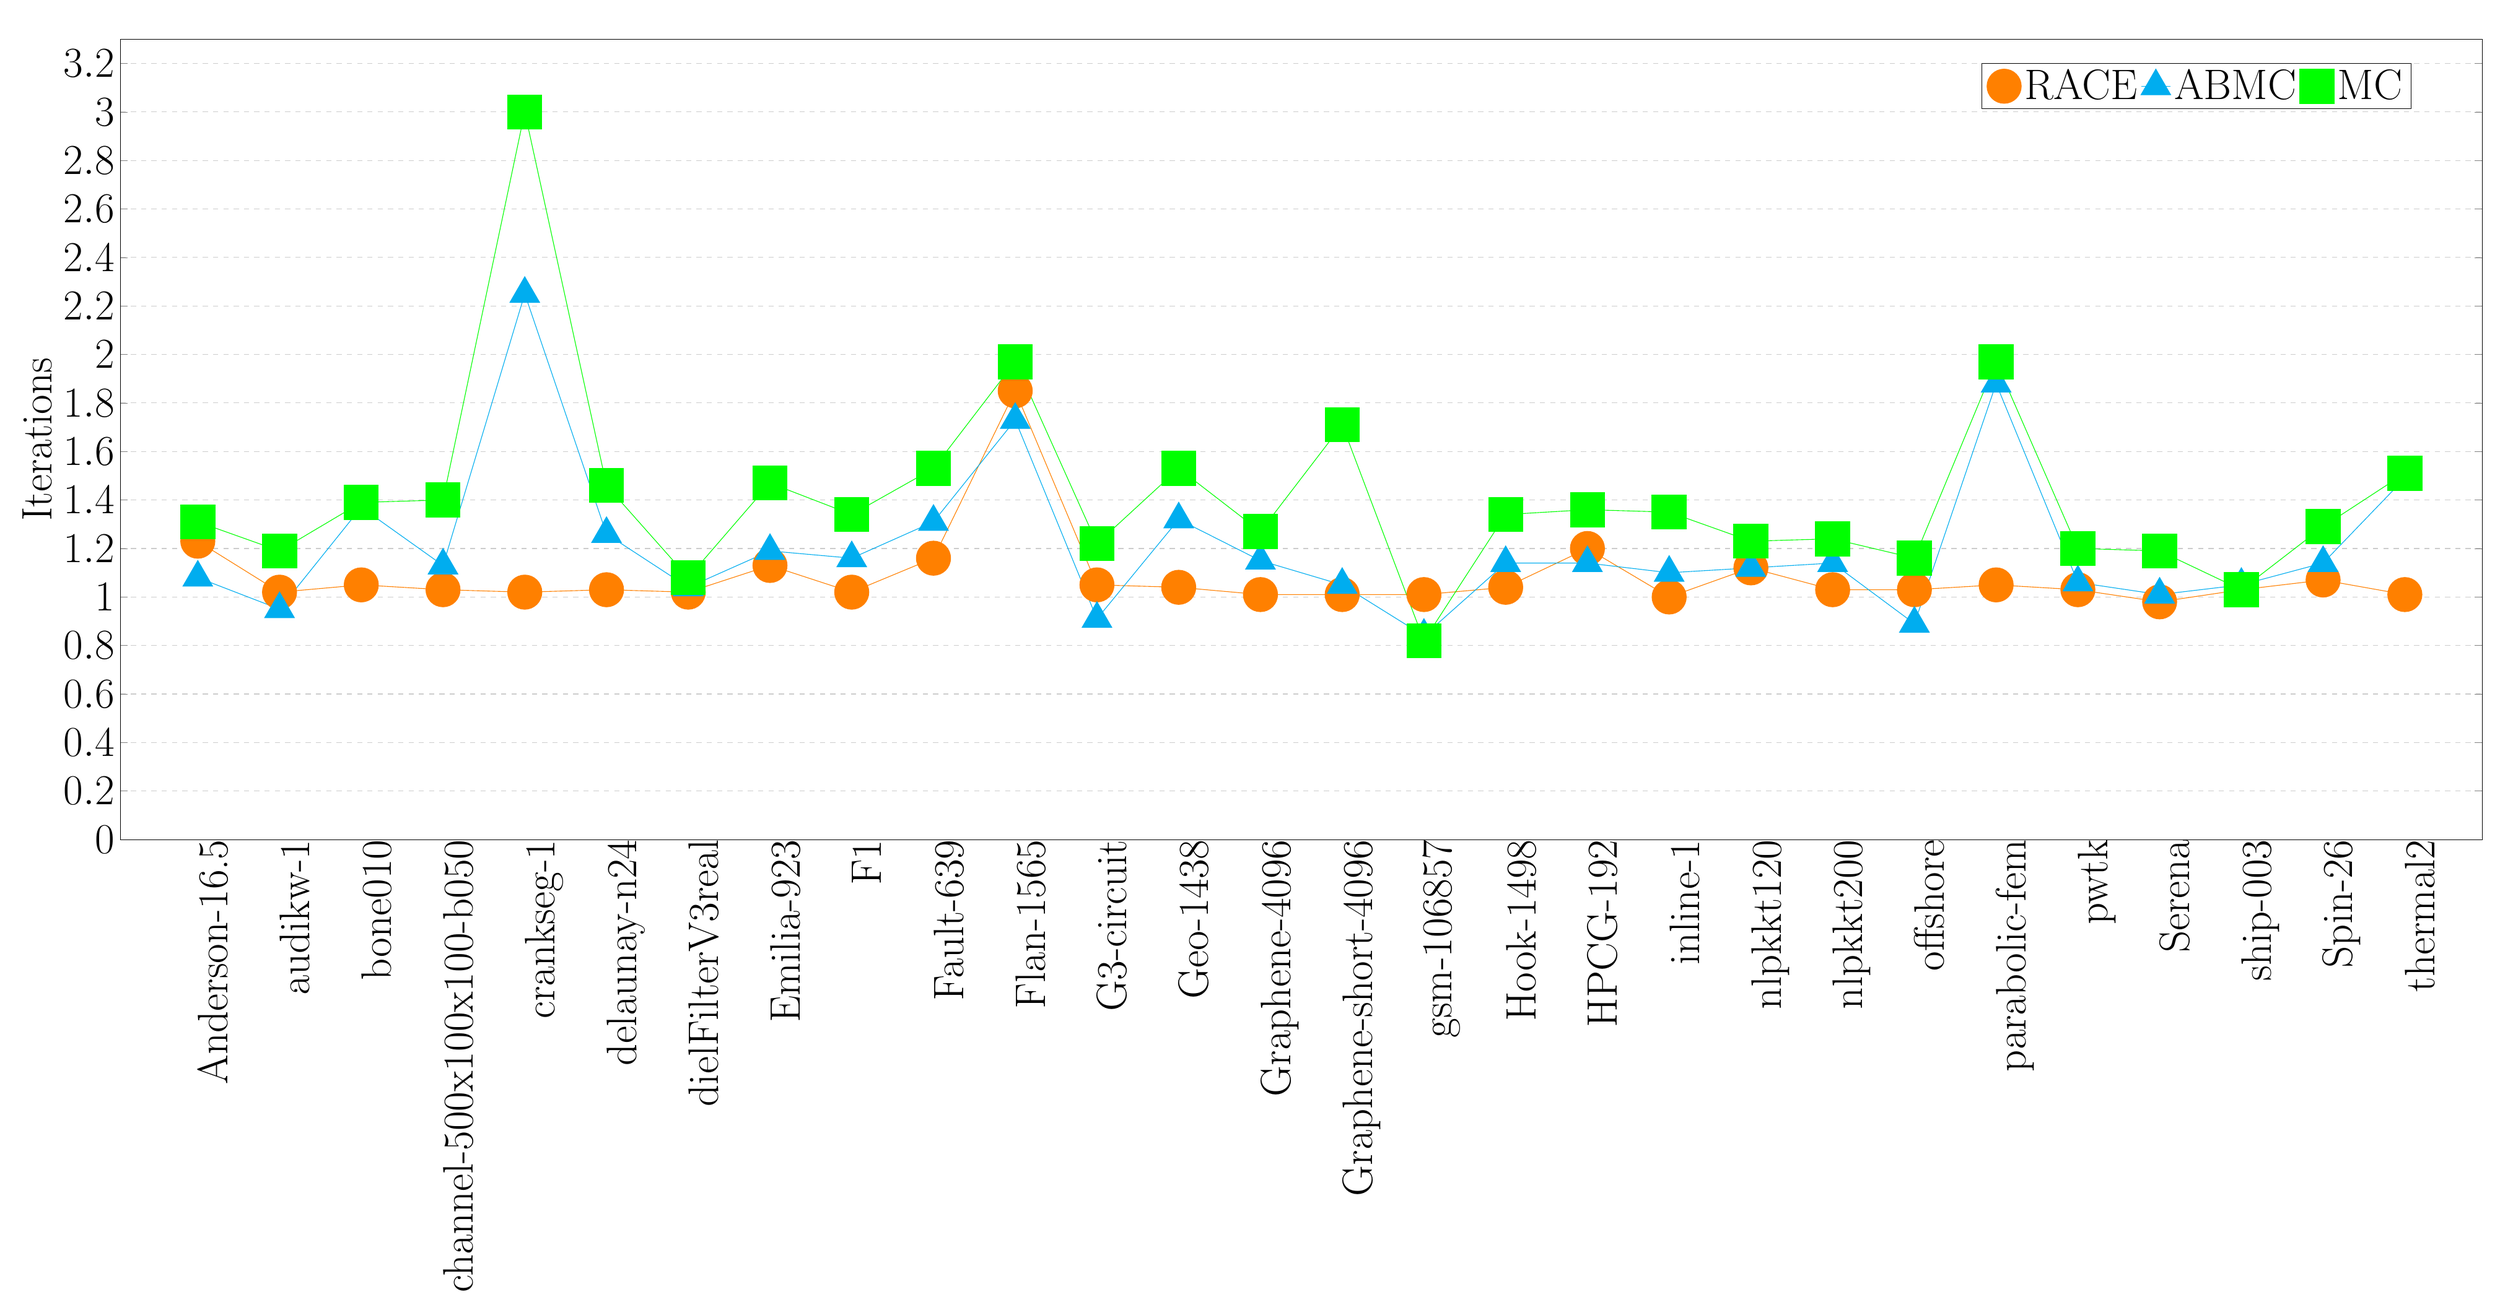
\begin{tikzpicture}
		%	\node at (13.25,15) {\LARGE{}};
			\begin{axis}[
		%	xmin=0.25, xmax=7.25,
			ymin=0, %ymax=3.25,
			xtick={1, 2, 3, 4, 5, 6, 7, 8, 9, 10, 11, 12, 13, 14, 15, 16, 17, 18, 19, 20, 21, 22, 23, 24, 25, 26, 27, 28},
		%	ytick={0,0.5,1,1.5,2,2.5,3},
			xticklabels={Anderson-16.5, audikw-1, bone010, channel-500x100x100-b050, crankseg-1, delaunay-n24, dielFilterV3real, Emilia-923, F1, Fault-639, Flan-1565, G3-circuit, Geo-1438, Graphene-4096, Graphene-short-4096, gsm-106857, Hook-1498, HPCG-192, inline-1, nlpkkt120, nlpkkt200, offshore, parabolic-fem, pwtk, Serena, ship-003, Spin-26, thermal2},
			width  = 50cm,
			height = 18cm,
			major x tick style = transparent,
			%	minor ytick={1, 5, 10, 15, 20, 25, 30 ,35,40},
			grid = minor,	
			%add_bar_commands
			ymajorgrids = true,
			grid style={dashed, gray!40},
			ylabel = {\Huge{Iterations}},
		%	symbolic x coords={Graphene-2048-2048, Graphene-4096-4096, Spin-24-24-24},
			x tick label style={rotate=90, anchor=north east, inner sep=0mm, font={\Huge}},
			tick label style={font={\Huge}},
			scaled y ticks = false,
			enlarge x limits=0.035,
			legend cell align=left,
			legend style={font=\Huge},
			legend columns=-1,
			legend style={
				%at={(1,1.05)},
				%anchor=south east,
				%column sep=1ex,
				legend pos=north east
			},
			%spl_legend_code
			title= {\Huge\scalebox{1.5}{{}}}
			]

\addplot[mark=*, mark size=10pt, mark options={orange}, draw=orange , y filter/.code={\pgfmathparse{\pgfmathresult*0.001}\pgfmathresult}] plot coordinates{(1,1230) (2,1020) (3,1050) (4,1030) (5,1020) (6,1030) (7,1020) (8,1130) (9,1020) (10,1160) (11,1850) (12,1050) (13,1040) (14,1010) (15,1010) (16,1010) (17,1040) (18,1200) (19,1000) (20,1120) (21,1030) (22,1030) (23,1050) (24,1030) (25,980) (26,1030) (27,1070) (28,1010)};
\addplot[mark=triangle*, mark size=10pt, mark options={cyan}, draw=cyan , y filter/.code={\pgfmathparse{\pgfmathresult*0.001}\pgfmathresult}] plot coordinates{(1,1080) (2,950) (3,1370) (4,1130) (5,2250) (6,1260) (7,1040) (8,1190) (9,1160) (10,1310) (11,1730) (12,910) (13,1320) (14,1150) (15,1050) (16,840) (17,1140) (18,1140) (19,1100) (20,1120) (21,1140) (22,890) (23,1880) (24,1060) (25,1010) (26,1050) (27,1140) (28,1490)};
\addplot[mark=square*, mark size=10pt, mark options={green}, draw=green , y filter/.code={\pgfmathparse{\pgfmathresult*0.001}\pgfmathresult}] plot coordinates{(1,1310) (2,1190) (3,1390) (4,1400) (5,3000) (6,1460) (7,1080) (8,1470) (9,1340) (10,1530) (11,1970) (12,1220) (13,1530) (14,1270) (15,1710) (16,820) (17,1340) (18,1360) (19,1350) (20,1230) (21,1240) (22,1160) (23,1970) (24,1200) (25,1190) (26,1030) (27,1290) (28,1510)};
	%addplot cmd

	\legend{RACE, ABMC, MC}

	\end{axis}			
\end{tikzpicture}

\end{document}

